\section{Extended Benchmarks}
\label{app:zq-bench}

Times are in milliseconds unless stated otherwise. Section~\ref{sec:zq-platform} describes the laptop. For the calibrated and replayed books, we timed 20 runs per book and thread count for our Rust implementation and ten for our Noir implementation. For the Cboe-derived books we timed five runs per book and thread count for our Rust implementation and one eight-thread run per book for our Noir implementation.

\subsection{The Clearing Proof Against Ticks and Volume Width}

\textbf{Table 22.} Our Rust implementation on uniform books, 250 orders per batch, one thread.

\begingroup
\setlength{\tabcolsep}{1.5pt}\scriptsize
\begin{longtable}{@{}>{\raggedright\arraybackslash}p{0.1125\linewidth}>{\raggedright\arraybackslash}p{0.1125\linewidth}>{\raggedright\arraybackslash}p{0.1125\linewidth}>{\raggedright\arraybackslash}p{0.1125\linewidth}>{\raggedright\arraybackslash}p{0.1125\linewidth}>{\raggedright\arraybackslash}p{0.1125\linewidth}>{\raggedright\arraybackslash}p{0.1125\linewidth}>{\raggedright\arraybackslash}p{0.1125\linewidth}@{}}
\toprule
\(N\) & \(n\) & \(k_{in}\) & Commitments & Proof (B) & Prove & Verify & Decode \\
\midrule\endfirsthead
\toprule
\(N\) & \(n\) & \(k_{in}\) & Commitments & Proof (B) & Prove & Verify & Decode \\
\midrule\endhead
\bottomrule\endfoot
100 & 128 & 16 & 70 & 4,908 & 264 & 9.2 & 15.3 \\
100 & 128 & 32 & 97 & 6,636 & 349 & 10.2 & 21.1 \\
250 & 256 & 16 & 52 & 3,756 & 298 & 8.7 & 11.5 \\
250 & 256 & 32 & 79 & 5,484 & 448 & 9.6 & 17.5 \\
500 & 512 & 16 & 62 & 4,396 & 582 & 9.0 & 13.5 \\
500 & 512 & 32 & 89 & 6,124 & 781 & 9.7 & 19.0 \\
1,000 & 1,024 & 16 & 62 & 4,396 & 998 & 9.3 & 14.0 \\
1,000 & 1,024 & 32 & 89 & 6,124 & 1,366 & 10.0 & 19.3 \\
2,000 & 2,048 & 16 & 62 & 4,396 & 1,803 & 9.2 & 14.1 \\
2,000 & 2,048 & 32 & 89 & 6,124 & 2,462 & 10.0 & 19.6 \\
4,000 & 4,096 & 16 & 62 & 4,396 & 3,330 & 9.1 & 13.7 \\
4,000 & 4,096 & 32 & 89 & 6,124 & 4,506 & 10.1 & 19.2 \\
8,000 & 8,192 & 16 & 62 & 4,396 & 6,367 & 8.9 & 13.6 \\
8,000 & 8,192 & 32 & 89 & 6,124 & 8,723 & 9.8 & 18.9 \\
\end{longtable}
\endgroup

\begingroup
\setlength{\tabcolsep}{2pt}\small
\begin{longtable}{@{}>{\raggedright\arraybackslash}p{0.1500\linewidth}>{\raggedright\arraybackslash}p{0.1500\linewidth}>{\raggedright\arraybackslash}p{0.1500\linewidth}>{\raggedright\arraybackslash}p{0.1500\linewidth}>{\raggedright\arraybackslash}p{0.1500\linewidth}>{\raggedright\arraybackslash}p{0.1500\linewidth}@{}}
\toprule
\(N\) & \(n\) & \(k_{in}\) & Update-validity prove & No-cross prove & Batch check \\
\midrule\endfirsthead
\toprule
\(N\) & \(n\) & \(k_{in}\) & Update-validity prove & No-cross prove & Batch check \\
\midrule\endhead
\bottomrule\endfoot
100 & 128 & 16 & 378 & 92 & 77 \\
100 & 128 & 32 & 415 & 111 & 78 \\
250 & 256 & 16 & 384 & 118 & 78 \\
250 & 256 & 32 & 449 & 152 & 80 \\
500 & 512 & 16 & 381 & 190 & 77 \\
500 & 512 & 32 & 422 & 234 & 78 \\
1,000 & 1,024 & 16 & 382 & 320 & 78 \\
1,000 & 1,024 & 32 & 424 & 402 & 79 \\
2,000 & 2,048 & 16 & 625 & 568 & 80 \\
2,000 & 2,048 & 32 & 693 & 715 & 81 \\
4,000 & 4,096 & 16 & 1,102 & 1,047 & 85 \\
4,000 & 4,096 & 32 & 1,218 & 1,303 & 87 \\
8,000 & 8,192 & 16 & 1,950 & 1,950 & 95 \\
8,000 & 8,192 & 32 & 2,196 & 2,484 & 95 \\
\end{longtable}
\endgroup

\textbf{Table 23.} Our Rust implementation on the same books with eight threads.

\begingroup
\setlength{\tabcolsep}{1.5pt}\scriptsize
\begin{longtable}{@{}>{\raggedright\arraybackslash}p{0.1125\linewidth}>{\raggedright\arraybackslash}p{0.1125\linewidth}>{\raggedright\arraybackslash}p{0.1125\linewidth}>{\raggedright\arraybackslash}p{0.1125\linewidth}>{\raggedright\arraybackslash}p{0.1125\linewidth}>{\raggedright\arraybackslash}p{0.1125\linewidth}>{\raggedright\arraybackslash}p{0.1125\linewidth}>{\raggedright\arraybackslash}p{0.1125\linewidth}@{}}
\toprule
\(N\) & \(k_{in}\) & Prove & Verify & Decode & Update-validity prove & No-cross prove & Batch check \\
\midrule\endfirsthead
\toprule
\(N\) & \(k_{in}\) & Prove & Verify & Decode & Update-validity prove & No-cross prove & Batch check \\
\midrule\endhead
\bottomrule\endfoot
100 & 16 & 98 & 6.4 & 3.6 & 122 & 41 & 52 \\
100 & 32 & 117 & 6.7 & 5.0 & 131 & 50 & 53 \\
250 & 16 & 115 & 6.2 & 2.9 & 113 & 56 & 51 \\
250 & 32 & 154 & 6.4 & 3.9 & 122 & 72 & 51 \\
500 & 16 & 192 & 6.4 & 3.3 & 115 & 84 & 51 \\
500 & 32 & 236 & 6.7 & 4.6 & 123 & 102 & 52 \\
1,000 & 16 & 291 & 6.4 & 3.6 & 114 & 114 & 52 \\
1,000 & 32 & 376 & 6.7 & 4.8 & 122 & 128 & 52 \\
2,000 & 16 & 484 & 6.5 & 3.7 & 174 & 178 & 54 \\
2,000 & 32 & 615 & 6.8 & 4.7 & 190 & 215 & 54 \\
4,000 & 16 & 865 & 6.6 & 3.6 & 314 & 314 & 60 \\
4,000 & 32 & 1,081 & 6.6 & 4.6 & 314 & 354 & 60 \\
8,000 & 16 & 1,590 & 6.7 & 3.6 & 532 & 533 & 70 \\
8,000 & 32 & 2,026 & 6.8 & 4.6 & 549 & 618 & 69 \\
\end{longtable}
\endgroup

At \(n=256\), the accumulated widths of 24 and 40 bits are multiples of eight, so the proof needs no scaled top limbs. This explains the smaller column count than at \(n=512\). At \(n=128\) the prover uses seven-bit limbs and needs more columns. With 250 orders the update-validity domain has \(\max(n,1024)\) rows. Timings vary little up to \(n=1024\) and increase at larger \(n\). Using eight threads on four physical cores speeds up clearing-proof generation by a factor of 3.6 at \(n=1024\) and 4.3 at \(n=8192\).

\begin{figure}[!tp]
    \centering
    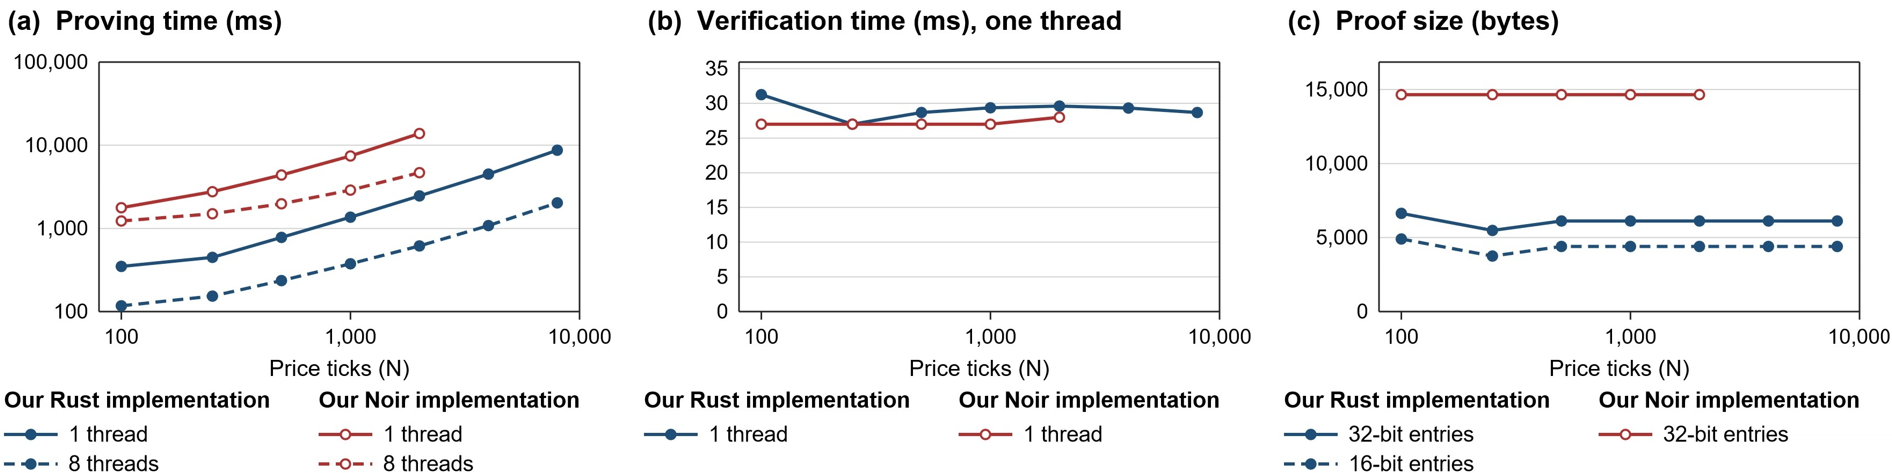
\includegraphics[width=\linewidth]{figures/fig3-performance.png}
    \caption{Scaling with price-grid size. Our Rust implementation uses uniform books and our Noir implementation uses calibrated books. Panel (a) shows proving time. For our Noir implementation it plots the median of the paired witness and proof times, whereas Table 5 sums the two component medians. Panel (b) shows one-thread verification, including decoding for our Rust implementation. Panel (c) gives the serialized proof size at the indicated input widths.}
    \label{fig:performance-scaling}
\end{figure}

\subsection{Spread}

\textbf{Table 24.} Our Rust implementation, \(N = 1000\), 32-bit volumes, 250 orders: median and interquartile range over 20 runs.

\begingroup
\setlength{\tabcolsep}{2pt}\small
\begin{longtable}{@{}>{\raggedright\arraybackslash}p{0.3960\linewidth}>{\raggedright\arraybackslash}p{0.2520\linewidth}>{\raggedright\arraybackslash}p{0.2520\linewidth}@{}}
\toprule
Metric & One thread & Eight threads \\
\midrule\endfirsthead
\toprule
Metric & One thread & Eight threads \\
\midrule\endhead
\bottomrule\endfoot
Clearing proof, prove & 1,366 [1,356--1,377] & 376 [359--384] \\
Clearing proof, verify & 10.0 [9.5--10.3] & 6.7 [6.6--6.8] \\
Clearing proof, decode & 19.3 [18.8--19.6] & 4.8 [4.5--5.2] \\
Update-validity proof, prove & 424 [419--428] & 122 [121--123] \\
Update-validity proof, verify & 43.0 [42.4--44.0] & 20.5 [20.0--20.8] \\
Batch check & 79.3 [77.5--80.3] & 52.0 [51.5--52.3] \\
\end{longtable}
\endgroup

All three proofs in the 1,000-tick, 32-bit configuration open at two points. The crossing, update-validity and no-cross proofs contain 89, 17 and 20 column-and-quotient commitments, respectively. In the eight-thread experiment of Table 4, update-proof verification including decoding took 23, 43 and 69 ms at 250, 1,000 and 2,200 orders. The update proof occupied 1,700 bytes at each log length. The full batch check in Table 24 uses decoded inputs.

\subsection{Calibrated and Replayed Books}

\textbf{Table 25.} Our Rust implementation's clearing proof on the calibrated books (five per size) and on the 32 replayed books, 32-bit volumes. Brackets give the range of the per-book medians.

\begingroup
\setlength{\tabcolsep}{2pt}\small
\begin{longtable}{@{}>{\raggedright\arraybackslash}p{0.1500\linewidth}>{\raggedright\arraybackslash}p{0.1500\linewidth}>{\raggedright\arraybackslash}p{0.1500\linewidth}>{\raggedright\arraybackslash}p{0.1500\linewidth}>{\raggedright\arraybackslash}p{0.1500\linewidth}>{\raggedright\arraybackslash}p{0.1500\linewidth}@{}}
\toprule
Books & \(N\) & \(n\) & Prove, one thread & Prove, eight threads & Verify + decode, one thread \\
\midrule\endfirsthead
\toprule
Books & \(N\) & \(n\) & Prove, one thread & Prove, eight threads & Verify + decode, one thread \\
\midrule\endhead
\bottomrule\endfoot
Calibrated & 100 & 128 & 343 [341--345] & 117 [111--130] & 30.6 \\
Calibrated & 250 & 256 & 414 [408--420] & 150 [134--156] & 26.3 \\
Calibrated & 500 & 512 & 769 [765--771] & 232 [228--235] & 28.6 \\
Calibrated & 1,000 & 1,024 & 1,343 [1,339--1,351] & 373 [363--382] & 28.8 \\
Calibrated & 2,000 & 2,048 & 2,437 [2,433--2,447] & 626 [608--633] & 28.6 \\
Replayed & 601--662 & 1,024 & 1,348 [1,334--1,363] & 367 [353--381] & 29.5 \\
\end{longtable}
\endgroup

At a domain size of 1,024, median clearing-proof generation times for the uniform, calibrated, and replayed books differ by less than 3\%.

On the 362 Cboe-derived books (101 ticks, 32-bit inputs), the median of the per-book proving medians for our Rust implementation was 384 ms on one thread and 112 ms on eight. Each clearing proof occupied 6,636 bytes.

\subsection{Operations Outside the Proofs}

\textbf{Table 26.} Per-order and per-batch operations in our Rust implementation, \(N = 1000\), 32-bit volumes.

\begingroup
\setlength{\tabcolsep}{2pt}\small
\begin{longtable}{@{}>{\raggedright\arraybackslash}p{0.3240\linewidth}>{\raggedright\arraybackslash}p{0.1530\linewidth}>{\raggedright\arraybackslash}p{0.1530\linewidth}>{\raggedright\arraybackslash}p{0.2700\linewidth}@{}}
\toprule
Operation & One thread & Eight threads & Encoded size \\
\midrule\endfirsthead
\toprule
Operation & One thread & Eight threads & Encoded size \\
\midrule\endhead
\bottomrule\endfoot
Record an order (exchange) & 0.98 & 0.99 & 416 B in the public log \\
Check a receipt (trader) & 0.24 & 0.24 & 192 B private receipt \\
Open a batch & 13.3 & 9.6 & 1,576 B \\
Check an opening & 19.1 & 18.5 &  \\
Run the clearing rule & 0.07 & 0.08 &  \\
\end{longtable}
\endgroup

The single-thread recording time of 0.98 ms per order corresponds to roughly 1,000 order updates per second for this operation alone.

\subsection{Our Noir Implementation}

\textbf{Table 27.} Our Noir implementation on the calibrated books (median over five books and ten runs each, interquartile range in brackets) and on the 32 replayed books. The proof is 14,656 bytes and verification takes 27 to 30 ms in every row.

\begingroup
\setlength{\tabcolsep}{1.5pt}\scriptsize
\begin{longtable}{@{}>{\raggedright\arraybackslash}p{0.1350\linewidth}>{\raggedright\arraybackslash}p{0.0990\linewidth}>{\raggedright\arraybackslash}p{0.1080\linewidth}>{\raggedright\arraybackslash}p{0.0900\linewidth}>{\raggedright\arraybackslash}p{0.0990\linewidth}>{\raggedright\arraybackslash}p{0.1080\linewidth}>{\raggedright\arraybackslash}p{0.1440\linewidth}>{\raggedright\arraybackslash}p{0.1170\linewidth}@{}}
\toprule
Books & \(N\) & Gates & Threads & Witness & Key & Prove & Prover memory \\
\midrule\endfirsthead
\toprule
Books & \(N\) & Gates & Threads & Witness & Key & Prove & Prover memory \\
\midrule\endhead
\bottomrule\endfoot
Calibrated & 100 & 12,757 & 1 & 720 & 344 & 1,052 [1,044--1,064] & 36 MB \\
 &  &  & 8 & 702 & 191 & 525 [518--540] & 45 MB \\
Calibrated & 250 & 27,357 & 1 & 764 & 683 & 1,994 [1,981--2,012] & 57 MB \\
 &  &  & 8 & 739 & 288 & 764 [754--777] & 68 MB \\
Calibrated & 500 & 51,666 & 1 & 844 & 1,181 & 3,541 [3,532--3,567] & 96 MB \\
 &  &  & 8 & 820 & 456 & 1,159 [1,145--1,173] & 106 MB \\
Calibrated & 1,000 & 100,357 & 1 & 1,001 & 2,213 & 6,427 [6,396--6,480] & 157 MB \\
 &  &  & 8 & 989 & 763 & 1,898 [1,879--1,927] & 180 MB \\
Calibrated & 2,000 & 197,666 & 1 & 1,337 & 4,260 & 12,478 [12,400--12,716] & 305 MB \\
 &  &  & 8 & 1,315 & 1,470 & 3,359 [3,333--3,420] & 326 MB \\
Replayed & 601--662 & 61,521--67,434 & 1 & 877 & 1,439 & 4,195 [4,115--4,300] & 116 MB \\
 &  &  & 8 & 858 & 537 & 1,316 [1,297--1,352] & 129 MB \\
\end{longtable}
\endgroup

The key column reports verification-key generation, performed once per book size. Additional threads accelerate proving, while witness generation remains sequential.

\textbf{Table 28.} Proving time for our Noir implementation, including witness generation, divided by proving time for our Rust implementation, on the same books.

\begingroup
\setlength{\tabcolsep}{2pt}\small
\begin{longtable}{@{}>{\raggedright\arraybackslash}p{0.3000\linewidth}>{\raggedright\arraybackslash}p{0.3000\linewidth}>{\raggedright\arraybackslash}p{0.3000\linewidth}@{}}
\toprule
\(N\) & One thread & Eight threads \\
\midrule\endfirsthead
\toprule
\(N\) & One thread & Eight threads \\
\midrule\endhead
\bottomrule\endfoot
100 & 5.2 & 10.5 \\
250 & 6.7 & 10.0 \\
500 & 5.7 & 8.5 \\
1,000 & 5.5 & 7.7 \\
2,000 & 5.7 & 7.5 \\
Replayed, 601--662 & 3.8 & 5.9 \\
\end{longtable}
\endgroup

Our Noir implementation runs as timed commands under WSL2, including process startup. For our Rust implementation we time native Windows function calls. The implementations also use different transcript hashes. We did not isolate these effects or benchmark another backend configuration.
